\documentclass{article}
\usepackage[preprint]{neurips_2025}
\usepackage[utf8]{inputenc}
\usepackage[T1]{fontenc}
\usepackage{hyperref,url,booktabs,amsfonts,amsmath,amssymb,nicefrac,microtype,xcolor,graphicx,enumitem}
\newcommand{\inprog}{\textcolor{orange!85!black}{[in progress]}}
\newcommand{\tbd}[1]{\textcolor{red!75!black}{[TBD: #1]}}

\title{You Get What You Verify: Physics Checkers Teach Small Models\\to Build Stable, Not Meaningful, LEGO}

\author{CS182 Project Team (4 members)\\University of California, Berkeley}

\begin{document}
\maketitle

\begin{abstract}
A recurring promise of AI for engineering is that an exact verifier --- a physics solver, a finite-element code --- can serve as an unlimited teacher: generate, check, keep what passes, learn from it. LEGO shrinks this promise to a setting where every structure can be checked for static equilibrium in seconds. We test it end to end. Large language models inside a physics-checking harness build structures that are both stable and recognizable (Claude Opus: 187/200 pass the checker; blind top-1 recognition 60--90\% against 75\% for dataset structures). But when this ability is handed to a small model, only the property the verifier checks survives. A 1.5B student distilled from 96 verified samples goes from 0/90 to 12/90 physics-valid designs, yet a blind judge recognizes \textbf{0/14} of its valid outputs, against 12/14 for matched dataset structures: it learned that stable means solid. In-context examples fare no better --- small models copy them verbatim. Scaling supervision to 4{,}000--4{,}852 examples raises physics validity to 15--26/90 (Gurobi-checked), yet across all four larger students \textbf{0/82} valid structures are recognized; and a size-matched control shows no detectable difference between verified AI-built data and the same amount of dataset data (B: 26 and 20 over two seeds; C: 21), so the teacher is not the bottleneck: the training signal is. The commonly used shape metric, voxel IoU, cannot see this failure (random dataset pairs score 0.151, no lower than real outputs). We conclude that a physics verifier teaches stability reliably and teaches nothing it does not check; design-capable small models need verifiers of intent, and we pre-specify two experiments to test this.
\end{abstract}

\section{Introduction}
\label{sec:intro}
Engineering design is a loop of proposing and checking. A structural engineer sketches a frame and runs an analysis; an architect's drawing goes to a structural check before it is built. The dream of AI-assisted design is to close this loop automatically and at scale: let a model propose, let an exact solver verify, and let the model learn from the verified proposals until it designs well on its own. The verifier never tires, never lies, and costs only compute. This is the premise behind reinforcement learning from verifiable rewards and behind rejection-sampling distillation, and it is why physics-checked generation has become an attractive testbed.

LEGO is the smallest honest instance of this premise. A brick layout stands only if contact and stud forces can balance gravity at every brick --- rigid-block equilibrium analysis, which shares its equilibrium equations with displacement-based finite-element analysis \cite{livesley1978,whiting2009} --- yet a $20^3$ layout can be checked by a linear program in seconds. BrickGPT \cite{pun2025brickgpt} showed that a 1B model trained on 47k stable layouts can generate text-conditioned designs, and follow-up work trains such models with physics rewards \cite{stable2026,pvpo2026}. These systems all rest on the same assumption: that a physics checker is a sufficient teacher.

We put that assumption under a microscope by asking a deliberately simple question: \emph{when the building ability of large models, exercised under a physics verifier, is transferred to a small model, what exactly transfers?}

\paragraph{Findings and contributions.}
\begin{enumerate}[leftmargin=*,itemsep=1pt]
\item \textbf{The teacher can build.} Large models in a generate$\rightarrow$verify$\rightarrow$repair harness produce structures that are physically valid and about as recognizable as dataset structures (\S\ref{sec:teacher}).
\item \textbf{Only what is verified transfers.} In-context examples make small models copy (\S\ref{sec:icl}). Distillation transfers stability (0$\rightarrow$12--26/90 valid) but not meaning: valid structures are recognized 0/14 times for the 96-sample student and 0/82 times for the 4k-example students (\S\ref{sec:distill},\S\ref{sec:meaning}).
\item \textbf{The teacher is not the bottleneck.} A pre-registered, size-matched control finds no detectable difference between verified AI data and dataset data (\S\ref{sec:distill}), so the limitation lies in what the training signal contains.
\item \textbf{Why this was easy to miss.} Voxel IoU, the usual shape metric, scores degenerate and good outputs alike; a blind recognition protocol separates them (\S\ref{sec:testbed}).
\item \textbf{What to do next.} We pre-specify two experiments that add a semantic verifier to the loop (\S\ref{sec:future}).
\end{enumerate}

\section{Related work}
\label{sec:related}
\paragraph{Physics-checked brick generation.}
Graphics work treated LEGO as optimization: Legolization \cite{luo2015legolization} converts meshes into brick layouts and repairs weak connections using a force-based stability analysis. Rigid-block equilibrium of this kind has a long history in structural engineering as limit analysis of masonry \cite{livesley1978} and has been used to generate structurally sound masonry buildings \cite{whiting2009}. BrickGPT \cite{pun2025brickgpt} made the problem a language-modeling one: each brick is a line \texttt{HxW (x,y,z)} on a $20^3$ grid; a Llama-3.2-1B model is fine-tuned on StableText2Brick (47k+ stable structures from 21 ShapeNet categories \cite{chang2015shapenet}, captioned by GPT-4o), and inference rejects colliding or floating bricks and rolls back to a stable prefix when a physics check fails (98.8\% stable with rollback, 24\% without). Its dataset is produced by voxelizing human-modeled meshes, not by hand-building. Later work removes the rollback by training with physics rewards \cite{stable2026,pvpo2026}; \cite{pvpo2026} names a failure mode closely related to ours, physically valid structures that do not match the target shape. LLaMA-Mesh \cite{wang2024llamamesh} shows more generally that LLMs can emit 3D geometry as text. Our contribution is not a better generator but a measurement of \emph{what such verifier-driven pipelines transfer} to a small model.

\paragraph{Agentic building and voxel worlds.}
BrickBench/BrickAgent \cite{brickbench} evaluates large models writing programs against an official verifier for inventory, connectivity, collision and stability; BrickWright \cite{brickwright} adds an agent workflow with part exploration, validation and visual rendering. In Minecraft, Voyager \cite{wang2023voyager} acquires skills through environment feedback and \cite{mcbuild2024} generates complete buildings from text. These works show that large models can build; they do not ask what survives transfer to small models.

\paragraph{Distillation and verifier-filtered data.}
Knowledge distillation trains a student on a teacher's outputs \cite{hinton2015distilling}; with black-box teachers the practical form is sequence-level distillation, fine-tuning on teacher-generated sequences \cite{kim2016sequence}, which can make a student \emph{better} than training on raw data because teacher outputs are more regular. DeepSeek-R1 distilled reasoning into 1.5B--70B students by SFT on 800k samples \cite{deepseekr1}. Filtering teacher samples with a verifier --- rejection-sampling fine-tuning \cite{yuan2023rft}, self-taught bootstrapping \cite{zelikman2022star}, Self-Instruct-style filters \cite{wang2023selfinstruct} --- is standard where answers can be checked. In mathematics the verifier checks exactly what is wanted (the answer). In design it does not: a physics checker verifies one necessary property of a good design. Our results show what happens in that gap.

\paragraph{In-context learning, feedback, and judges.}
Iterative self-correction with verbal feedback improves large models when the feedback is informative \cite{madaan2023selfrefine,shinn2023reflexion}. To measure semantics we use a VLM/LLM judge \cite{zheng2023judging}; such judges may prefer outputs of their own family \cite{panickssery2024selfpref}, which we mitigate with blind, shuffled renders and report as a limitation. Volumetric recognition work found that $30^3$--$32^3$ grids retain much category information while some classes become confusable \cite{wu2015shapenets,maturana2015voxnet,riegler2017octnet}; our $20^3$ setting is coarser, and we measure recognizability directly.

\section{Testbed and measurements}
\label{sec:testbed}
\paragraph{Task.} We keep BrickGPT's representation for comparability. A structure is a list of bricks $b_i=(h_i,w_i,x_i,y_i,z_i)$, one per line, from a fixed library ($1\times1$ to $2\times6$ and rotations) on a $20^3$ grid. Input is a single caption with no examples. Students are evaluated one-shot ($k{=}0$) on 90 held-out captions (30 small, 30 medium, 30 large) and on 28 captions from four categories absent from StableText2Brick (airplane, house, tree, lamp). ``Dataset structures'' below are StableText2Brick layouts.

\paragraph{Physics verifier.} Checks run cheapest first: format, bounds, collision (no voxel occupied twice), floating (every brick connected to the ground; this alone is the \emph{connectivity} checker), and static stability following \cite{pun2025brickgpt,luo2015legolization}. For stability we seek contact and stud forces $\mathbf f_c$ such that for every brick $i$
\begin{equation}
\textstyle\sum_{c\ni i} \mathbf f_c + m_i\mathbf g = \mathbf 0,\qquad
\sum_{c\ni i} (\mathbf p_c-\mathbf o_i)\times \mathbf f_c = \mathbf 0,\qquad
\mathbf f_c \in \mathcal F_c ,
\label{eq:equil}
\end{equation}
with $\mathbf p_c$ the contact point, $\mathbf o_i$ the centre of mass and $\mathcal F_c$ the admissible set (compression unbounded, stud tension bounded). This linear feasibility problem is solved with Gurobi \cite{gurobi}. Cloud GPUs lack the Gurobi licence, so every reported number is re-checked locally with Gurobi.

\paragraph{Why not IoU.} The obvious semantic metric is aligned voxel IoU with the caption's reference structure \cite{stable2026}. It cannot do the job: physics-valid DeepSeek outputs score 0.134--0.155, randomly paired dataset structures score \textbf{0.151}, degenerate outputs score 0.167, and IoU separates degenerate from good structures with AUROC 0.43--0.63. A caption admits many correct proportions, so IoU mostly measures whether the generator guessed the reference's proportions.

\paragraph{Blind recognition.} Each structure is rendered from two fixed views with axes fixed to $[0,20]^3$; renders are shuffled under a hidden mapping and a judge $J$ (Claude) names its top-2 categories among the 21 before the mapping is read. With labels $y_i$,
\begin{equation}
\mathrm{Acc@}k=\frac1N\sum_{i}\mathbf 1\!\left[y_i\in \mathrm{top}\text{-}k\,J(r_i)\right],\qquad
\mathrm{VR}=\frac1{N}\sum_{i}\mathbf 1\!\left[\mathrm{valid}_i \wedge y_i=\mathrm{top}\text{-}1\,J(r_i)\right],
\end{equation}
where ``valid and recognized'' (VR) keeps a fixed denominator. Chance top-1 is $1/21\approx4.8\%$.

\section{The teacher can build}
\label{sec:teacher}
\begin{figure}[t]
\centering
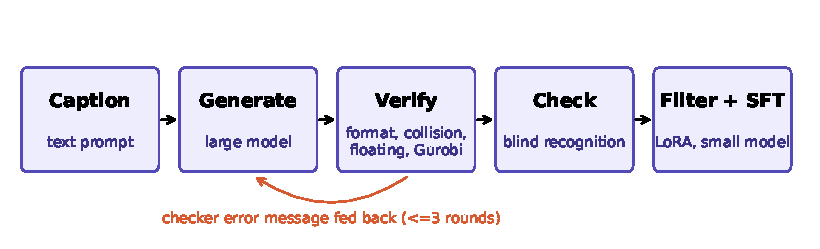
\includegraphics[width=\linewidth]{figs/pipeline.pdf}
\caption{Harness and distillation pipeline. A large model generates a brick list from a caption; the verifier checks format, bounds, collisions, floating bricks and static stability; failures are returned as text for up to 3 repair rounds. Accepted structures are filtered and used to fine-tune a small model with LoRA.}
\label{fig:pipeline}
\end{figure}

We first establish the ceiling: can large models, under the verifier, build both stably and meaningfully? We built our own harness (Figure~\ref{fig:pipeline}) so that every intermediate input and output is visible and reusable as training data. Text feedback from the verifier (e.g.\ ``brick 17 collides with brick 4 at (6,3,2)'') lifts deepseek-chat from 6/23 to 12/23 valid and deepseek-flash from 14/20 to 20/20. Claude Opus, writing a parametric voxel design per caption that a support-aware tiler converts to bricks, passes the verifier on 187/200 dataset captions and 59/60 new-category captions (Figure~\ref{fig:gallery}). These structures are also recognizable (Figure~\ref{fig:recog}): blind top-1 is 70\% for both DeepSeek harness arms, 60\% for the DeepSeek data later used for distillation, and 90\% for Opus, against 75\% for random dataset structures; the Opus figure is likely inflated by judge self-preference \cite{panickssery2024selfpref}. The teacher, in short, is both stable and meaningful. Its meaning comes from pre-training; the verifier only checked its stability.

\begin{figure}[t]
\centering
\begin{minipage}[t]{0.52\linewidth}\vspace{0pt}
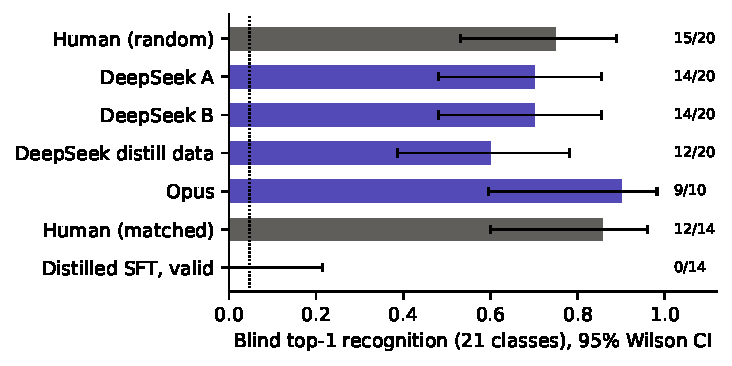
\includegraphics[width=\linewidth]{figs/recognition.pdf}
\end{minipage}\hfill
\begin{minipage}[t]{0.45\linewidth}\vspace{0pt}
\caption{Blind top-1 recognition among 21 classes with 95\% Wilson intervals (Appendix~\ref{app:stats}); dotted line: chance. Teacher outputs are about as recognizable as dataset structures; the \emph{physics-valid} outputs of the distilled student are never recognized.}
\label{fig:recog}
\end{minipage}
\end{figure}

\begin{figure}[t]
\centering
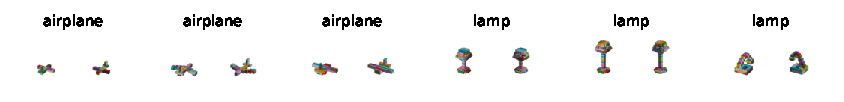
\includegraphics[width=\linewidth]{figs/opus_gallery.pdf}
\caption{Teacher structures (Claude Opus + support-aware tiler) for categories absent from StableText2Brick; all pass Gurobi.}
\label{fig:gallery}
\end{figure}

\section{Transfer by examples: the student copies}
\label{sec:icl}
The cheapest transfer channel is to show the student the teacher's work. Two team members tested this on BrickBench, where the model writes a Python build program checked by the official verifier, with Qwen2.5-Coder-1.5B-Instruct on 20 tasks each. In \emph{imitate} (two reference programs for the same task), zero-shot solved 0/20; two-shot solved 1--4/20 in one attempt and 6--7/20 with up to three rounds of error feedback, but every valid output had line similarity $>0.95$ to an example --- it was copied. In \emph{combine} (merge two works into a new target), zero-shot returned no code (0/20); two-shot returned code for 15/20 and passed physics on 3/20, all three byte-identical to one example, with 0/20 achieving the combination. A third team member ran the same idea with a large model (DeepSeek in BrickWright, 20 combination tasks): examples raised completion from 85\% to 100\% and reduced decision turns, without improving semantic scores or blind preference. Examples transfer shortcuts, not ability.

\section{Transfer by distillation: stability transfers}
\label{sec:distill}
If examples are copied, the next channel is to train on them. We fine-tune Qwen2.5-1.5B-Instruct \cite{qwen25} with LoRA \cite{hu2022lora} on caption$\rightarrow$brick-list pairs (hyperparameters in Appendix~\ref{app:hparams}).

\paragraph{Small distillation.} Training on 96 verified DeepSeek samples (12 optimizer steps) raises valid outputs from 0/90 to 12/90 (14/90 with checker feedback).

\paragraph{Pre-registered mixed-data comparison.} To give the student more supervision we compare group A, 4{,}000 dataset structures, with group B, the same 4{,}000 plus 284 verified AI-built structures (187 Opus, 65 DeepSeek, 32 Opus new-category) upsampled $\times3$ (4{,}852 examples); both run 304 optimizer steps from the same base. Decision rules were fixed before any output was downloaded (Appendix~\ref{app:prereg}). Because B also has more data than A, we added a pre-registered control C: the same 4{,}000 plus 284 \emph{additional dataset} structures upsampled $\times3$, matching B in size, repetition and steps, so that B and C differ only in where the extra structures came from.

\begin{figure}[t]
\centering
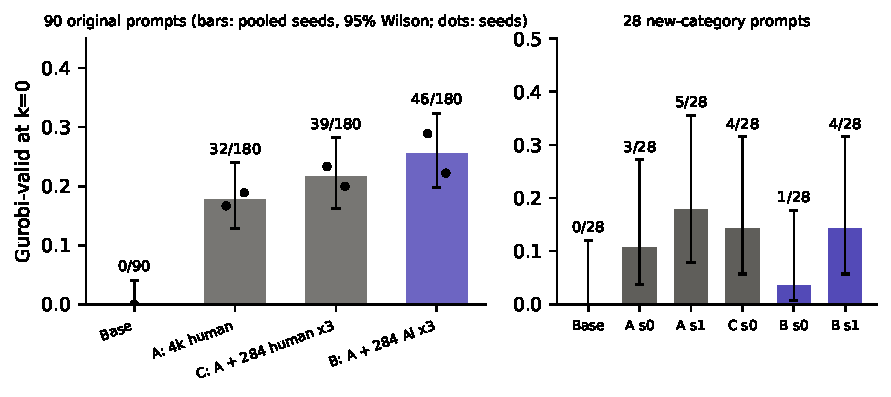
\includegraphics[width=\linewidth]{figs/physics_valid.pdf}
\caption{Gurobi-checked valid rate at $k{=}0$ with 95\% Wilson intervals. Left: 90 prompts from the 21 original categories. Right: 28 new-category prompts. All bars use Qwen2.5-1.5B; A, B, C differ only in training data (\S\ref{sec:distill}).}
\label{fig:valid}
\end{figure}

\paragraph{Results.} Figure~\ref{fig:valid} shows the Gurobi-checked counts with 95\% Wilson intervals. Every trained student is far above the untrained base (0/90 [0\%, 4\%]): A reaches 15/90 [10\%, 26\%] (Fisher $p=3\times10^{-5}$ vs.\ base); B reaches 26/90 [21\%, 39\%] (seed 0) and 20/90 [15\%, 32\%] (seed 1); C reaches 21/90 [16\%, 33\%] (seed 0). None of the data comparisons is significant: B seed 0 vs.\ A, one-sided $p=0.037$, two-sided $p=0.075$; B seed 1 vs.\ A, $p=0.45$; C vs.\ A, $p=0.35$; B seed 0 vs.\ C, $p=0.50$; B seed 1 vs.\ C, $p=1.0$; B pooled over two seeds (46/180) vs.\ C, two-sided $p=0.77$. The two seeds of B alone differ by 6 structures ($p=0.39$). Adding data gives a small, unstable gain, and there is no detectable difference between AI and dataset sources: verified AI-built data behaves as a substitute for dataset data, and the sequence-level-distillation hypothesis that teacher outputs are easier to fit \cite{kim2016sequence} finds no support at this scale. Most failures are collisions: 70 of A's 75 failures, 53 and 55 of B's 64 and 70, and 55 of C's 69. Training curves of all four runs are nearly identical (Figure~\ref{fig:curve}). Additional seeds (\tbd{A seed 1, C seed 1}) and held-out validation loss (\tbd{validation loss of the adapters on 200 held-out structures}) will complete this comparison.

\begin{figure}[t]
\centering
\begin{minipage}[t]{0.42\linewidth}\vspace{0pt}
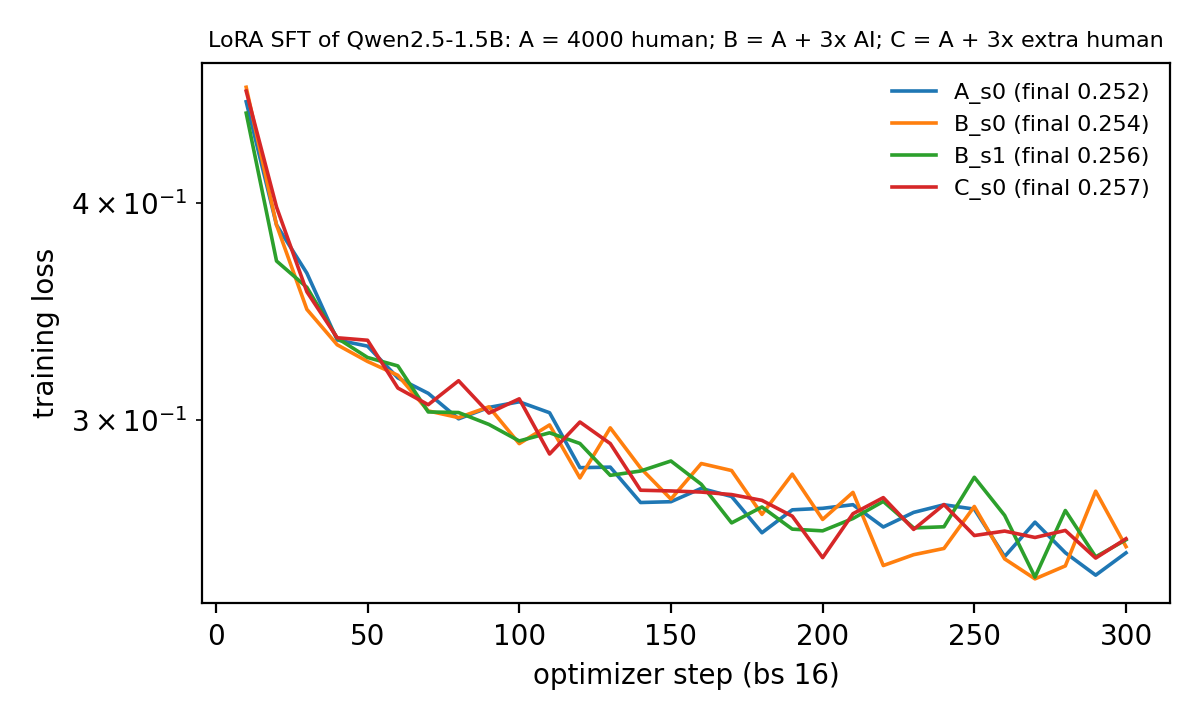
\includegraphics[width=\linewidth]{figs/train_curves.png}
\end{minipage}\hfill
\begin{minipage}[t]{0.55\linewidth}\vspace{0pt}
\caption{Training loss (token cross-entropy) of A, B (two seeds) and C over 304 steps; effective batch 16, cosine schedule. All runs fall from about 0.45--0.47 to about 0.25, so the groups fit their data equally well; held-out validation loss is \tbd{validation loss}. Token loss is a weak proxy here: the 96-sample student reached 0.227 yet produced unrecognizable structures.}
\label{fig:curve}
\end{minipage}
\end{figure}

\section{What does not transfer: meaning}
\label{sec:meaning}
Physics validity rose; did the students learn to build what was asked? No. For the 96-sample student (Figures~\ref{fig:recog},\ref{fig:solid}). Of its 14 valid structures, a blind judge recognized \textbf{0/14} at top-1 or top-2, versus 12/14 (top-2 13/14) for dataset structures of the same categories; six were called ``tower''. None passed the diversity filter that its own training data had passed. The student found the cheapest route to validity --- a compact solid post or block --- even though its training data were recognizable (60\% top-1). The teacher's meaning did not transfer; only the verified property did. The gap (0/14 vs.\ 12/14) is far larger than the sampling noise of this small set.

The larger students tell the same story at larger scale. Across A, B (two seeds) and C, the 82 physics-valid structures on the 90 prompts were judged blind under the same protocol: \textbf{0/82} recognized at top-1 and 1/82 at top-2. Almost all are two to four parallel vertical columns, occasionally a wall slab or a solid block: the cheapest stable answer, learned regardless of whether the extra data came from the teacher or from the dataset. On the 28 new-category prompts, the 12 valid structures were recognized once (a lamp from C); the pre-registered primary metric, valid-and-recognized out of 28, is A 0, B 0 (both seeds), C 1, all within two of the base, so by our pre-registered rule new categories are \emph{not learnable at this scale}. All recognition judgments come from a single judge (Claude), and the valid structures are highly uniform; both are limitations.

\begin{figure}[t]
\centering
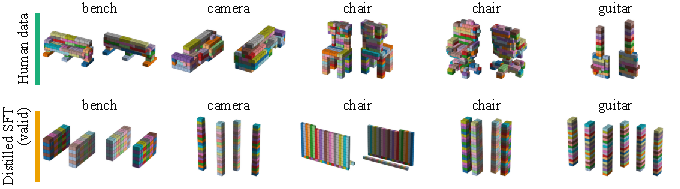
\includegraphics[width=0.92\linewidth]{figs/solid_vs_human.pdf}
\caption{Top: dataset structures of the same categories (12/14 recognized). Bottom: physics-valid outputs of the 96-sample distilled student (0/14 recognized) --- posts, slabs and blocks. Titles are ground-truth categories.}
\label{fig:solid}
\end{figure}

\section{Discussion: you get what you verify}
\label{sec:discussion}
Across every channel, the student acquired the cheapest regularity that satisfies the check it is trained or evaluated against. With examples it copies (\S\ref{sec:icl}); with distillation it learns that solid stacks stand (\S\ref{sec:meaning}); in a teammate's distillation of multi-step BrickWright agent trajectories (275 teacher trajectories into Qwen3.5-2B), the student completed 0/10 tasks, mostly repeating actions in loops. Two explanations are ruled out by our controls: the teacher is not at fault, since the teacher's own outputs are recognizable and the dataset-data control behaves like AI data; and fit is not at fault, since all groups reach the same training loss. What remains is the signal: our pipeline filters and evaluates on physics, so physics is what is taught and measured. The teacher is meaningful because of its pre-training, not because of the verifier, and that meaning does not survive a few thousand verified examples. In engineering terms, a stability solver certifies that a design will not fall down; it says nothing about whether it is the bridge you asked for. A pipeline that learns only from the solver will, given the chance, design the solid block.

\paragraph{Limitations.} Evaluation sets are small (14--90 items); most comparisons have one or two seeds; the semantic judge is a model from the same family as one generator; new-category captions were written by a model; the team's experiments use different representations (brick tokens vs.\ build programs) and are compared qualitatively; and all students are LoRA-tuned 1.5B models trained for one pass, so our claims are restricted to this low-compute regime.

\section{Conclusion}
\label{sec:conclusion}
A physics verifier is a reliable teacher of stability: across distillation settings it took a small model from 0 to 12--26 valid designs out of 90. It teaches nothing it does not check: none of the 96 valid structures produced by our students was recognizable at top-1: whether the design is the object described was never in the signal, and it did not transfer --- worse, the verifier invited a solution that satisfies the check and means nothing. For small models to learn to design, the verifier must cover design intent.

\section{Future work: training with a semantic verifier}
\label{sec:future}
We pre-specify, but did not run for lack of time, two experiments that turn our blind-recognition metric into a training signal and pair it with the physics verifier.
\begin{enumerate}[leftmargin=*,itemsep=1pt]
\item \textbf{Semantic filtering of distillation data.} Keep only teacher samples that are physics-valid \emph{and} recognized at top-1 by the VLM judge; compare against physics-only filtering at equal size and steps. Prediction: similar valid rates, markedly higher recognition of valid outputs. Criterion: VR on the 90 prompts increases with one-sided Fisher $p<0.05$.
\item \textbf{Dual-verifier reward.} After SFT, apply rejection sampling or RL with reward $=\mathbf 1[\text{valid}]\cdot\mathbf 1[\text{recognized}]$. Risk: the VLM judge can itself be gamed; evaluation will therefore use a different VLM than the reward, plus human spot checks.
\end{enumerate}

\bibliographystyle{plain}
\bibliography{refs}

\appendix
\section{Research log}
\label{app:log}
This appendix records, in order, the questions we asked, the experiments we ran and why we changed course (full record in \texttt{results/RESEARCH\_TRAJECTORY.md}).
\begin{enumerate}[leftmargin=*,itemsep=1pt]
\item \textbf{Original proposal (rejected).} Adding new brick types and physics to a generator; judged too hard for our compute. The GSI suggested a smaller ICL question on bridges.
\item \textbf{Can a model ``grow up'' and need its verifier less?} Qwen SFT on 4{,}000 dataset structures reached about 10\% valid (10/90 with Gurobi for Qwen3.5-2B), reproducing BrickGPT's order of magnitude; official BrickGPT weights reached 20/90. A planned RL stage was paused for lack of compute.
\item \textbf{Does the \emph{content} of error feedback matter?} Four pre-registered arms trained from scratch on successes, trial-and-error traces with checker feedback, the same traces with shuffled feedback, and retries without feedback (3 seeds each). $k{=}0$ success was 1.35\%, 0.40\%, 0.48\% and 0.87\% with overlapping intervals: no detectable difference; recorded as a negative result.
\item \textbf{A conservative stability screener, and the finite-element replication.} A small GNN screener with a one-sided conformal guarantee \cite{angelopoulos2021gentle} kept its guarantee on 19 of 21 held-out LEGO categories. On real trusses analysed with our own finite-element solver, only part of the structure families kept it; the Howe-truss failure traced to a shape shortcut (the model associated the Pratt silhouette with ``safe''), and diagonal-flip augmentation reduced Howe's miss rate from 31.8\% to 1.5\%. A mechanism-based warning signal did not work. This line is outside the main story but shows the same pattern: the model learned the cheapest available regularity.
\item \textbf{ICL on BrickBench} (\S\ref{sec:icl}): copying.
\item \textbf{Team decision: harness + distillation}, after the GSI emphasized that the course requires training by gradient descent.
\item \textbf{DeepSeek in the harness, and a voided vision test.} Rendered views as feedback first looked worse than text, until we found the renderer auto-scaled each axis; the test was voided and renders now use fixed axes. A data-budget overrun (\textyen5.04 against \textyen5) led to in-round balance checks.
\item \textbf{IoU dropped} (\S\ref{sec:testbed}); a first recognition run was voided because two processes wrote into the same directory.
\item \textbf{12/90 that turned out to be solid blocks} (\S\ref{sec:meaning}). We first read 12/90 as a positive result; looking at the renders revealed the shortcut and motivated the blind protocol.
\item \textbf{Mixed data and the size-matched control} (\S\ref{sec:distill}). The first Kaggle submissions failed at bootstrap (auto-extracted archive, missing parent directory) and were fixed before resubmission. Noticing that B had more data than A led to control C.
\item \textbf{Gemini as a teacher.} Gemini 3.8 Flash produced 665 verified structures paired with dataset captions, but they are systematically squatter than dataset structures (median longest/shortest side 1.6 vs.\ 2.6; only 254/665 within 30\% of the dataset proportions). The teacher's style bias would be inherited; we stopped before training on them.
\end{enumerate}

\section{Pre-registered decision rules}
\label{app:prereg}
A/B (fixed before download): primary metric VR on the 28 new-category prompts; ``B helps'' requires a difference $\ge5$ and one-sided Fisher $p<0.05$; on the 90 prompts, ``no harm'' requires B $\ge$ A$-5$ with two-sided $p\ge0.05$; any group within 2 of the base on new categories ``learned nothing''. Outcome: new categories, valid-and-recognized A 0, B 0, C 1 of 28 --- ``not learnable at this scale''; on the 90 prompts B is not worse than A (two-sided $p=0.075$), so ``no harm'' holds. Control C (fixed before any C result): ``AI source helps'' requires mean B $-$ mean C $\ge5$ and one-sided $p<0.05$; ``only amount'' requires C $-$ A $\ge5$ and $|B-C|<5$. Current outcome (one seed of C): C $-$ A $=6$, mean B $-$ C $=2$; neither rule's significance condition is met (C vs.\ A $p=0.35$), so the provisional verdict is ``no reliable difference''; final verdict after \tbd{A seed 1, C seed 1}. Connectivity-checker numbers (Kaggle): A 17/90, B 27/90 (seed 0) and 22/90 (seed 1), C 21/90; new categories A 4, B 1 and 4, C 4 (/28).

\section{Hyperparameters}
\label{app:hparams}
\begin{table}[h]
\centering\small
\begin{tabular}{@{}lll@{}}
\toprule
Setting & Value & Rationale \\
\midrule
Base model & Qwen2.5-1.5B-Instruct & largest Qwen that trains with LoRA on a free 16\,GB T4 \\
LoRA rank & 16 & common default \cite{hu2022lora} \\
Learning rate & $2\times10^{-4}$, cosine & standard LoRA SFT rate; not tuned (compute) \\
Batch & 2 $\times$ 8 accumulation = 16 & fits T4 memory with 3{,}072-token sequences \\
Max length & 3{,}072 tokens & covers almost all examples \\
Steps (A/B/C) & 304 & $\lceil 4852/16\rceil$; identical for all groups to fix compute \\
Steps (96-sample distill) & 12 (2 epochs) & all data available; under-training diagnosed post hoc \\
AI / extra-data upsampling & $\times3$ & 284 extra structures become $\sim$18\% of B and C \\
Grid / bricks & $20^3$, BrickGPT library & comparability with \cite{pun2025brickgpt} \\
Teacher repair rounds & $\le 3$ & cost control; most repairs happen in round 1 \\
Student decoding & one-shot, $k{=}0$ & isolates what is in the weights \\
\bottomrule
\end{tabular}
\end{table}

\section{Error bars and tests}
\label{app:stats}
All rates are binomial proportions over small sets, so we report 95\% Wilson score intervals \cite{wilson1927}: for $k$ successes in $n$ trials, $\hat p=k/n$, the interval is
$\bigl(\hat p+\tfrac{z^2}{2n}\pm z\sqrt{\hat p(1-\hat p)/n+z^2/4n^2}\bigr)/(1+z^2/n)$ with $z=1.96$; unlike the normal approximation it stays in $[0,1]$ and is reliable at $k=0$, which occurs often here. Group comparisons use Fisher's exact test on $2\times2$ tables, exact for small counts. These intervals capture sampling noise over prompts, not seed variance; where two seeds exist we report both, and the 6-structure difference between B's seeds ($p=0.39$) shows seed variance is of the same order as the effects we test.

\section{Reproducibility}
Code, data-generation scripts, evaluation and \texttt{paper/make\_figs.py} (regenerating every figure from result files) are in the team repository, branch \texttt{lego-distill}, directory \texttt{distill/}; the public release is \tbd{public repository}. StableText2Brick is public and fetched by script; AI-generated structures are included as JSONL; the Kaggle code bundle is public as \texttt{brickexp-code-public}.

\end{document}
